\documentclass{article}

\usepackage{pgfplots}
\pgfplotsset{compat=1.18}
\usepackage[a4paper,margin=0.4cm]{geometry}
\usepgfplotslibrary{groupplots}

% ================= COLOR + MARKER CYCLE =================
\pgfplotscreateplotcyclelist{crda_rda_cycle}{
% --- CRDA ---
{blue,   solid,  mark=*},
{red,    solid,  mark=square*},
{brown,  solid,  mark=triangle*},
% --- RDA ---
{green,  solid, mark=*},
{gray,   solid, mark=square*},
{purple, solid, mark=triangle*},
}

\begin{document}

\begin{figure*}[t]
\centering

% ================= GLOBAL LEGEND =================
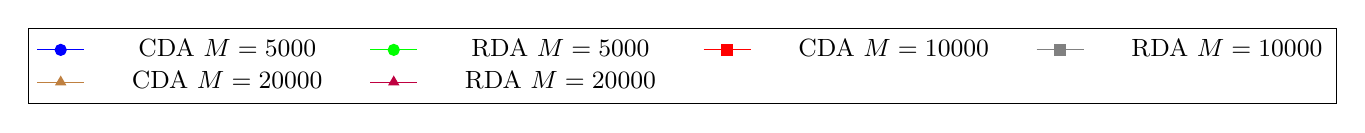
\begin{tikzpicture}
\begin{axis}[
    hide axis,
    xmin=0, xmax=1,
    ymin=0, ymax=1,
    legend columns=4,
    legend style={
        draw,
        at={(0.5,0)},
        anchor=north,
        column sep=1.5em,
        font=\small
    },
]
\addlegendimage{blue,   solid,  mark=*}
\addlegendentry{CDA $M = 5000$}
\addlegendimage{green,  solid, mark=*}
\addlegendentry{RDA $M = 5000$}

\addlegendimage{red,    solid,  mark=square*}
\addlegendentry{CDA $M = 10000$}
\addlegendimage{gray,   solid, mark=square*}
\addlegendentry{RDA $M = 10000$}

\addlegendimage{brown,  solid,  mark=triangle*}
\addlegendentry{CDA $M = 20000$}
\addlegendimage{purple, solid, mark=triangle*}
\addlegendentry{RDA $M = 20000$}
\end{axis}
\end{tikzpicture}

\vspace{0.4cm}

% =========================================================
% ==================== 2 x 3 SUBPLOTS  ====================
% =========================================================

\begin{tikzpicture}
\begin{groupplot}[
    group style={
        group size=2 by 4,
        horizontal sep=1.6cm,
        vertical sep=2.0cm
    },
    width=0.33\textwidth,
    height=4.8cm,
    grid=major,
    xmode=log,
    ymode=log,
    cycle list name=crda_rda_cycle,
]

%%%%%%%%%%%%%%%%%%%%%%%%%%%%%%%%%%%%%%%%%%%%%%%%%%%%%%%%%%%%
% ===================== EPS = 0.05 ========================
%%%%%%%%%%%%%%%%%%%%%%%%%%%%%%%%%%%%%%%%%%%%%%%%%%%%%%%%%%%%
% draw=none, mark=none, forget plot

% -------- k1 vs k2 --------
\nextgroupplot[
    xlabel={$k_2$},
    ylabel={},
    title={$k_1$},
]

\addplot+[mark repeat=20] table[x=k2,y=k1,col sep=comma]{results/cda/estimates_k_16_eps10_M5000.csv};
\addplot+[mark repeat=20] table[x=k2,y=k1,col sep=comma]{results/cda/estimates_k_16_eps10_M10000.csv};
\addplot+[mark repeat=20] table[x=k2,y=k1,col sep=comma]{results/cda/estimates_k_16_eps10_M20000.csv};
\addplot+[draw=none, mark=none, forget plot] table[x=k2,y=k1,col sep=comma]{results/rda/estimates_data_eps10_M5000.csv};
\addplot+[draw=none, mark=none, forget plot] table[x=k2,y=k1,col sep=comma]{results/rda/estimates_data_eps10_M10000.csv};
\addplot+[draw=none, mark=none, forget plot] table[x=k2,y=k1,col sep=comma]{results/rda/estimates_data_eps10_M20000.csv};

\nextgroupplot[
    xlabel={$k_2$},
    ylabel={},
    title={$k_1$},
    cycle list shift=3,
]

\addplot+[draw=none, mark=none, forget plot] table[x=k2,y=k1,col sep=comma]{results/cda/estimates_k_16_eps10_M5000.csv};
\addplot+[draw=none, mark=none, forget plot] table[x=k2,y=k1,col sep=comma]{results/cda/estimates_k_16_eps10_M10000.csv};
\addplot+[draw=none, mark=none, forget plot] table[x=k2,y=k1,col sep=comma]{results/cda/estimates_k_16_eps10_M20000.csv};
\addplot+[mark repeat=20] table[x=k2,y=k1,col sep=comma]{results/rda/estimates_data_eps10_M5000.csv};
\addplot+[mark repeat=20] table[x=k2,y=k1,col sep=comma]{results/rda/estimates_data_eps10_M10000.csv};
\addplot+[mark repeat=20] table[x=k2,y=k1,col sep=comma]{results/rda/estimates_data_eps10_M20000.csv};

% -------- Duplication --------
\nextgroupplot[
    xlabel={$k_2$},
    ylabel={},
    title={Replication Factor},
]
\addplot+[mark repeat=20] table[x=k2,y=replication_factor,col sep=comma]{results/cda/estimates_k_16_eps10_M5000.csv};
\addplot+[mark repeat=20] table[x=k2,y=replication_factor,col sep=comma]{results/cda/estimates_k_16_eps10_M10000.csv};
\addplot+[mark repeat=20] table[x=k2,y=replication_factor,col sep=comma]{results/cda/estimates_k_16_eps10_M20000.csv};
\addplot+[draw=none, mark=none, forget plot] table[x=k2,y=replication_factor,col sep=comma]{results/rda/estimates_data_eps10_M5000.csv};
\addplot+[draw=none, mark=none, forget plot] table[x=k2,y=replication_factor,col sep=comma]{results/rda/estimates_data_eps10_M10000.csv};
\addplot+[draw=none, mark=none, forget plot] table[x=k2,y=replication_factor,col sep=comma]{results/rda/estimates_data_eps10_M20000.csv};

\nextgroupplot[
    xlabel={$k_2$},
    ylabel={},
    title={Replication Factor},
    cycle list shift=3,
]
\addplot+[draw=none, mark=none, forget plot] table[x=k2,y=replication_factor,col sep=comma]{results/cda/estimates_k_16_eps10_M5000.csv};
\addplot+[draw=none, mark=none, forget plot] table[x=k2,y=replication_factor,col sep=comma]{results/cda/estimates_k_16_eps10_M10000.csv};
\addplot+[draw=none, mark=none, forget plot] table[x=k2,y=replication_factor,col sep=comma]{results/cda/estimates_k_16_eps10_M20000.csv};
\addplot+[mark repeat=20] table[x=k2,y=replication_factor,col sep=comma]{results/rda/estimates_data_eps10_M5000.csv};
\addplot+[mark repeat=20] table[x=k2,y=replication_factor,col sep=comma]{results/rda/estimates_data_eps10_M10000.csv};
\addplot+[mark repeat=20] table[x=k2,y=replication_factor,col sep=comma]{results/rda/estimates_data_eps10_M20000.csv};

% -------- Store Complexity --------
\nextgroupplot[
    xlabel={$k_2$},
    ylabel={},
    title={Probagation Cost},
]
\addplot+[mark repeat=20] table[x=k2,y=probagation_complexity,col sep=comma]{results/cda/estimates_k_16_eps10_M5000.csv};
\addplot+[mark repeat=20] table[x=k2,y=probagation_complexity,col sep=comma]{results/cda/estimates_k_16_eps10_M10000.csv};
\addplot+[mark repeat=20] table[x=k2,y=probagation_complexity,col sep=comma]{results/cda/estimates_k_16_eps10_M20000.csv};
\addplot+[draw=none, mark=none, forget plot] table[x=k2,y=probagation_complexity,col sep=comma]{results/rda/estimates_data_eps10_M5000.csv};
\addplot+[draw=none, mark=none, forget plot] table[x=k2,y=probagation_complexity,col sep=comma]{results/rda/estimates_data_eps10_M10000.csv};
\addplot+[draw=none, mark=none, forget plot] table[x=k2,y=probagation_complexity,col sep=comma]{results/rda/estimates_data_eps10_M20000.csv};

\nextgroupplot[
    xlabel={$k_2$},
    ylabel={},
    title={Probagation Cost},
    cycle list shift=3,
]
\addplot+[draw=none, mark=none, forget plot] table[x=k2,y=probagation_complexity,col sep=comma]{results/cda/estimates_k_16_eps10_M5000.csv};
\addplot+[draw=none, mark=none, forget plot] table[x=k2,y=probagation_complexity,col sep=comma]{results/cda/estimates_k_16_eps10_M10000.csv};
\addplot+[draw=none, mark=none, forget plot] table[x=k2,y=probagation_complexity,col sep=comma]{results/cda/estimates_k_16_eps10_M20000.csv};
\addplot+[mark repeat=20] table[x=k2,y=probagation_complexity,col sep=comma]{results/rda/estimates_data_eps10_M5000.csv};
\addplot+[mark repeat=20] table[x=k2,y=probagation_complexity,col sep=comma]{results/rda/estimates_data_eps10_M10000.csv};
\addplot+[mark repeat=20] table[x=k2,y=probagation_complexity,col sep=comma]{results/rda/estimates_data_eps10_M20000.csv};

% -------- Store Complexity --------
\nextgroupplot[
    xlabel={$k_2$},
    ylabel={},
    title={Historical Synchronization Cost},
]
\addplot+[mark repeat=20] table[x=k2,y=historical_synchronization_complexity,col sep=comma]{results/cda/estimates_k_16_eps10_M5000.csv};
\addplot+[mark repeat=20] table[x=k2,y=historical_synchronization_complexity,col sep=comma]{results/cda/estimates_k_16_eps10_M10000.csv};
\addplot+[mark repeat=20] table[x=k2,y=historical_synchronization_complexity,col sep=comma]{results/cda/estimates_k_16_eps10_M20000.csv};
\addplot+[draw=none, mark=none, forget plot] table[x=k2,y=historical_synchronization_complexity,col sep=comma]{results/rda/estimates_data_eps10_M5000.csv};
\addplot+[draw=none, mark=none, forget plot] table[x=k2,y=historical_synchronization_complexity,col sep=comma]{results/rda/estimates_data_eps10_M10000.csv};
\addplot+[draw=none, mark=none, forget plot] table[x=k2,y=historical_synchronization_complexity,col sep=comma]{results/rda/estimates_data_eps10_M20000.csv};

\nextgroupplot[
    xlabel={$k_2$},
    ylabel={},
    title={Historical Synchronization Cost},
    cycle list shift=3,
]
\addplot+[draw=none, mark=none, forget plot] table[x=k2,y=historical_synchronization_complexity,col sep=comma]{results/cda/estimates_k_16_eps10_M5000.csv};
\addplot+[draw=none, mark=none, forget plot] table[x=k2,y=historical_synchronization_complexity,col sep=comma]{results/cda/estimates_k_16_eps10_M10000.csv};
\addplot+[draw=none, mark=none, forget plot] table[x=k2,y=historical_synchronization_complexity,col sep=comma]{results/cda/estimates_k_16_eps10_M20000.csv};
\addplot+[mark repeat=20] table[x=k2,y=historical_synchronization_complexity,col sep=comma]{results/rda/estimates_data_eps10_M5000.csv};
\addplot+[mark repeat=20] table[x=k2,y=historical_synchronization_complexity,col sep=comma]{results/rda/estimates_data_eps10_M10000.csv};
\addplot+[mark repeat=20] table[x=k2,y=historical_synchronization_complexity,col sep=comma]{results/rda/estimates_data_eps10_M20000.csv};
\end{groupplot}
\end{tikzpicture}

\caption{
Comparison between RobustCDA and RDA across
$N \in \{2500, 5000, 10000\}$.
(Top row) $\epsilon = 0.05$,
(Bottom row) $\epsilon = 0.10$.
Columns show $k_1$ vs $k_2$, data duplication, and storage complexity.
}
\end{figure*}

\end{document}